
\subsection{Material Properties and Geometry}

Figure~\ref{fig:skew_quad_geometry_ansys} presents a cross-section of the skew quadrupole used for a magnetic analysis. The iron yoke, the coil, and the remaining parts of the model considered as air are marked in red, blue, and violet respectively. The~magnet cross-section has three axes of symmetry. Therefore, only one-eighth of the skew quadrupole is simulated.  

\begin{figure}[H]
    \centering
    \begin{tikzpicture}[scale=0.8]
    \node[scale=0.8] at (0,0) {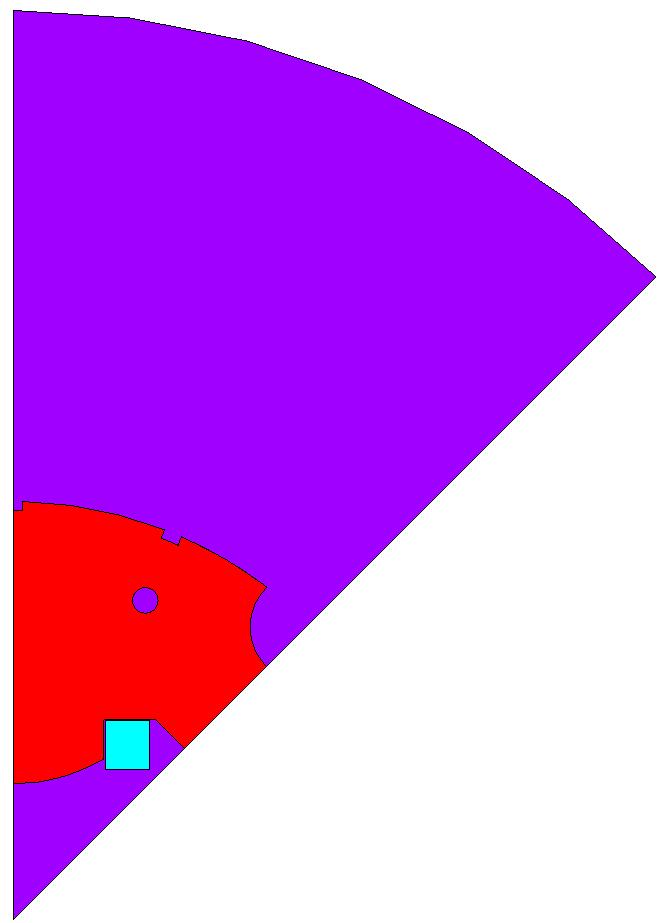
\includegraphics[width=.3\textwidth]{sections/skew_quad_q_det/figures/magnetic_map/skew_quad_geometry.png}};

    \draw[black, thick, ->] (2.5,0) -- (-1.1,0);
    \draw[black, thick, ->] (2.5,-0.95) -- (-1.32,-0.95);
    \draw[black, thick, ->] (2.5,-1.5) -- (-1,-1.5);
    \draw[black, thick, ->] (2.5,-2) -- (-1.4,-2);
    \draw[black, thick, ->] (2.5,-2.5) -- (-1.8,-2.5);
    
    \draw[red, dashed] (-2.35,-3.3) -- (2.5,-3.3);
    \draw[red, dashed] (-2.3,-3.3) -- (-2.3,3.3);
    \draw[red, dashed] (-2.35,-3.45) -- (2.8,1.67);
    \node[red, scale=0.8] at (3.5,1.9) {axes of symmetry};
    
    \node[black, scale=0.8] at (3.5,0) {air external};
    \node[black, scale=0.8] at (3.5,-0.95) {air hole};
    \node[black, scale=0.8] at (3.5,-1.5) {iron yoke};
    \node[black, scale=0.8] at (3.5,-2) {coil};
    \node[black, scale=0.8] at (3.5,-2.5) {air internal};

    \end{tikzpicture}
    \caption{The \nth{8} part of the skew quadrupole cross-section with specified component names.}
    \label{fig:skew_quad_geometry_ansys}
\end{figure}

The~coil cross-section is homogenised magnetically and electrically, i.e. there is no distinction between the insulation and the strand composite. In the magnetic analysis of the~skew quadrupole, it is assumed that the magnet is infinitely long. This assumption allows for considering this case as a plane 2D problem. The areas considered as air and the~coil are characterised by the magnetic relative permeability equal to one. The iron yoke is characterised by a~non-linear B-H curve, as presented in Fig.~\ref{fig:b_h_curve}. 

\begin{figure}[H]
    \centering
    \begin{tikzpicture}
        \begin{axis}[
          width=0.7\linewidth, 
          height = 4.0cm,
          xlabel={$H,~\text{A/m}$},
          ylabel={$B,~\text{T}$},
          ymax=3.0,
          ]
          \addplot[smooth, blue] table[x=h,y=b,col sep=comma] {sections/skew_quad_q_det/figures/magnetic_map/bh_curve.csv}; 
    \end{axis}
    \end{tikzpicture}
    \caption{B-H curve of an iron yoke of the skew quadrupole.}
    \label{fig:b_h_curve}
\end{figure}


\subsection{Mesh, Initial and Boundary Conditions}

The meshed geometry is illustrated in Fig~\ref{fig:skew_quad_magnetic_mesh_ansys}. The element PLANE233 is used for the analysis. It is a 2-D element for simulating 2D planar and axisymmetric magnetic fields. The element is defined by 8 nodes~\cite{ansys_element_manual}.

\begin{figure}[H]
    \centering
    \begin{tikzpicture}[scale=0.9]
    \node[scale=0.9] at (0,0) {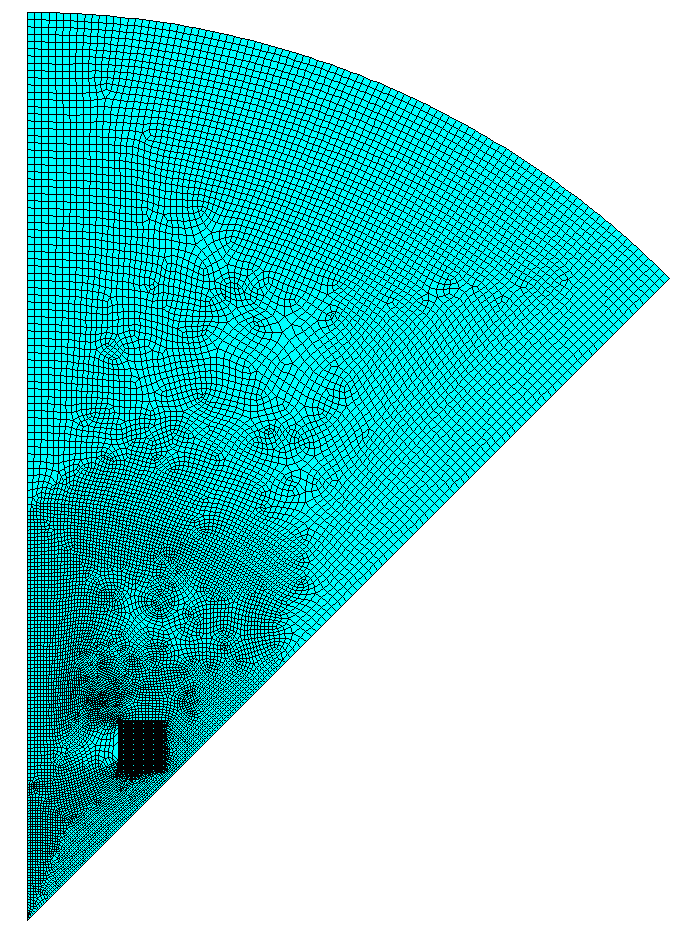
\includegraphics[width=.3\textwidth]{sections/skew_quad_q_det/figures/magnetic_map/skew_quad_mesh.png}};
    \node[scale=0.9] at (5,0) {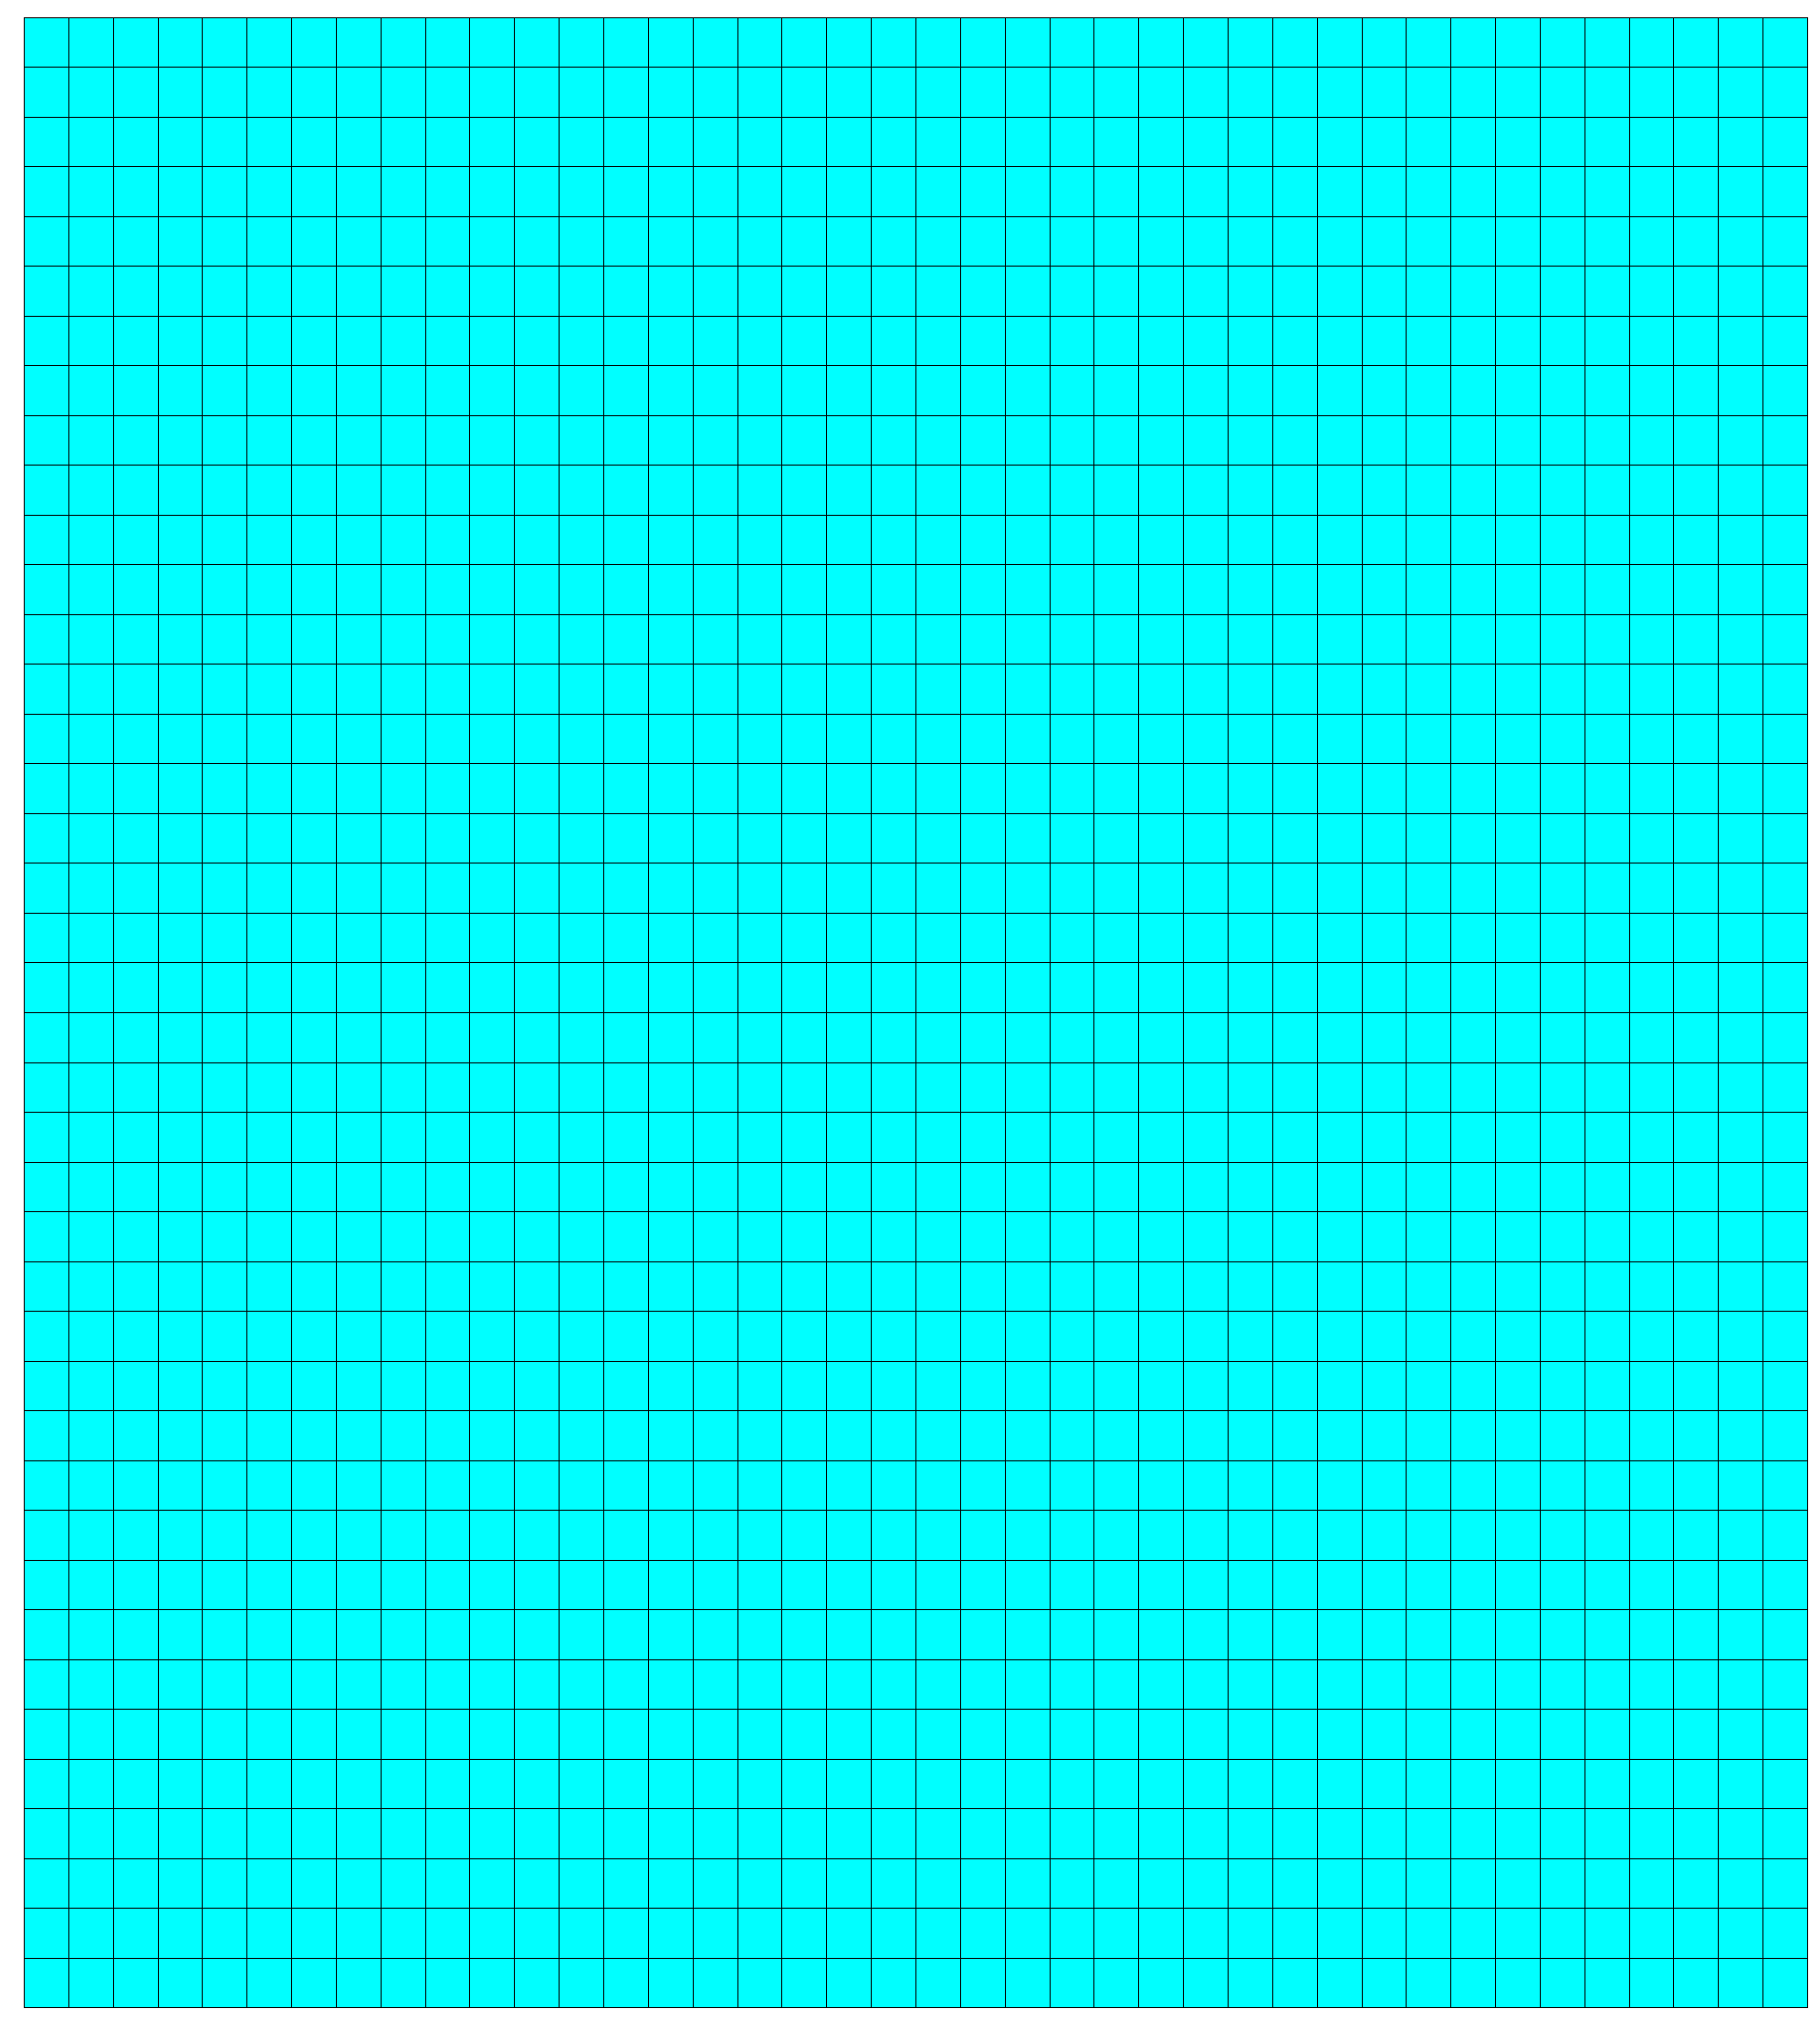
\includegraphics[width=.25\textwidth]{sections/skew_quad_q_det/figures/magnetic_map/skew_quad_mesh_coil.png}};
    \draw[red, very thick, dashed] (-2.3,-3.1) -- (-2.3,3.1);
    \node[red, scale=0.8] at (-3,2) {$A_\text{z}=0$};
    
    \draw[black, very thick, ->] (-0.9,-1.9) -- (3.0,0);
    \node[black, scale=0.8] at (5,2.5) {Mesh in the coil};
    
    \draw[scale=1] (-3.5,1-1) circle (0.1cm);
    \draw[black, ->, scale=1] (-3.5,1-1) -- (-3.5,1.5-1);
    \draw[black, ->, scale=1] (-3.5,1-1) -- (-3,1-1);
    \node[scale = 0.8] at (-3.75,0.8-1) {$\vec{z}$};
    \node[scale = 0.8] at (-2.9,1.2-1) {$\vec{x}$};
    \node[scale = 0.8] at (-3.7,1.65-1) {$\vec{y}$};
    
    \end{tikzpicture}
    \caption{The \nth{8} part of the skew quadrupole cross-section.}
    \label{fig:skew_quad_magnetic_mesh_ansys}
\end{figure}

For the requirements of the given analysis, the degrees of freedom only related to the~magnetic vector potential $A_\text{z}$ are used. In order to take into consideration the symmetry condition, the~magnetic vector potential $A_\text{z}$ is set to zero on the left side of the geometry. It means that the directional magnetic field $B_\text{x}$ is equal to zero on the left side marked in red. On the other side of the symmetry axis, it is assumed by default in ANSYS APDL that the magnetic flux is perpendicular to the wall. As illustrated in Fig~\ref{fig:skew_quad_magnetic_mesh_ansys}, the mesh is refined inside of the coil. There are 40 elements placed on each side of a rectangular area. The element size in the remaining components of the model is depicted in Table~\ref{table:mesh_characteristics_magnetic_ansys}.

\begin{table}[H]
    \caption{Mesh size characteristics of the skew quadrupole.} 
    \vspace{-1.em} 
    \fontsize{10}{10}
    \selectfont 
    \renewcommand{\arraystretch}{1.5}
    \begin{center}
        \begin{tabular}{ ccc } 
        \hline
        area name & element size & unit \\
        \hline
        iron yoke & 2 & mm \\
        air internal & 1.5 & mm \\
        air external & 4 & mm \\
        air hole & 2 & mm \\
        \hline 
        \end{tabular}
    \end{center}  
     \label{table:mesh_characteristics_magnetic_ansys} 
\end{table}

The uniformly distributed current density is applied to the coil area calculated as
\begin{equation}
    J_\text{coil} = \frac{n_\text{windings}~I}{A_\text{coil}},
\end{equation}
where $n_\text{windings}$ -- number of windings, $I$ -- current in each winding, $A_\text{coil}$ -- cross-sectional area of the coil with the resin and insulation. 86 static analyses are conducted with current linearly rising from 1 up to 86~A. 

\subsection{Results and Magnetic Field Mapping in the Skew Quadrupole}

Two values of current are chosen for the comparison of the magnetic field distribution inside the cross-section of the skew quadrupole, as shown in Fig.~\ref{fig:skew_quad_magnetic_results_geometry_ansys}. As expected, one can observe that the magnetic field increases with the rise of current. Moreover, the difference in the magnetic field distribution at different current levels is a result of the non-linear magnetic properties of the iron yoke.

\begin{figure}[H]
    \centering
    \begin{tikzpicture}
    \node at (0,0) {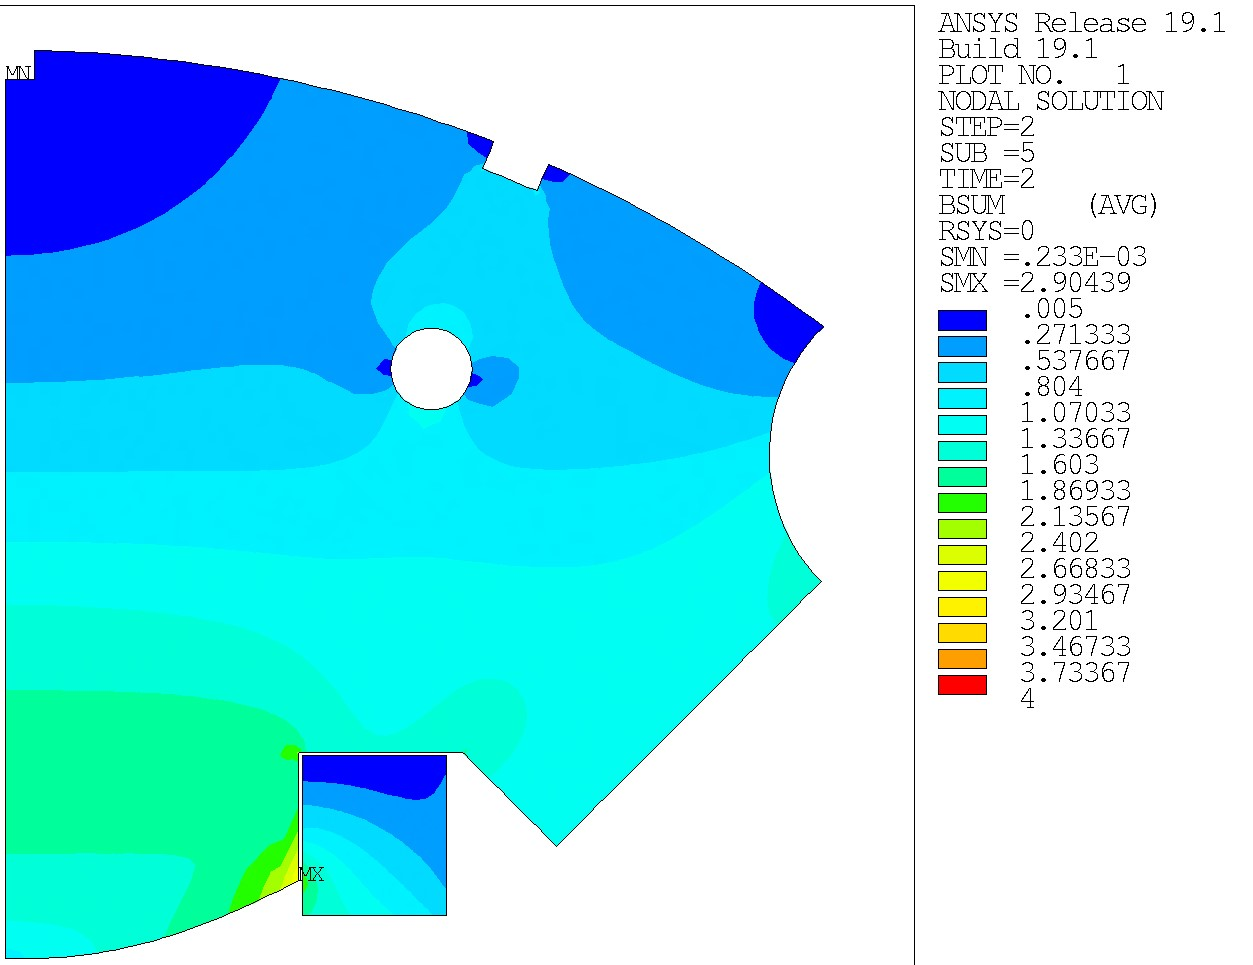
\includegraphics[width=.39\textwidth]{sections/skew_quad_q_det/figures/magnetic_map/peak_field_yoke_coil_current_40.jpg}};
    \node at (7.5,0) {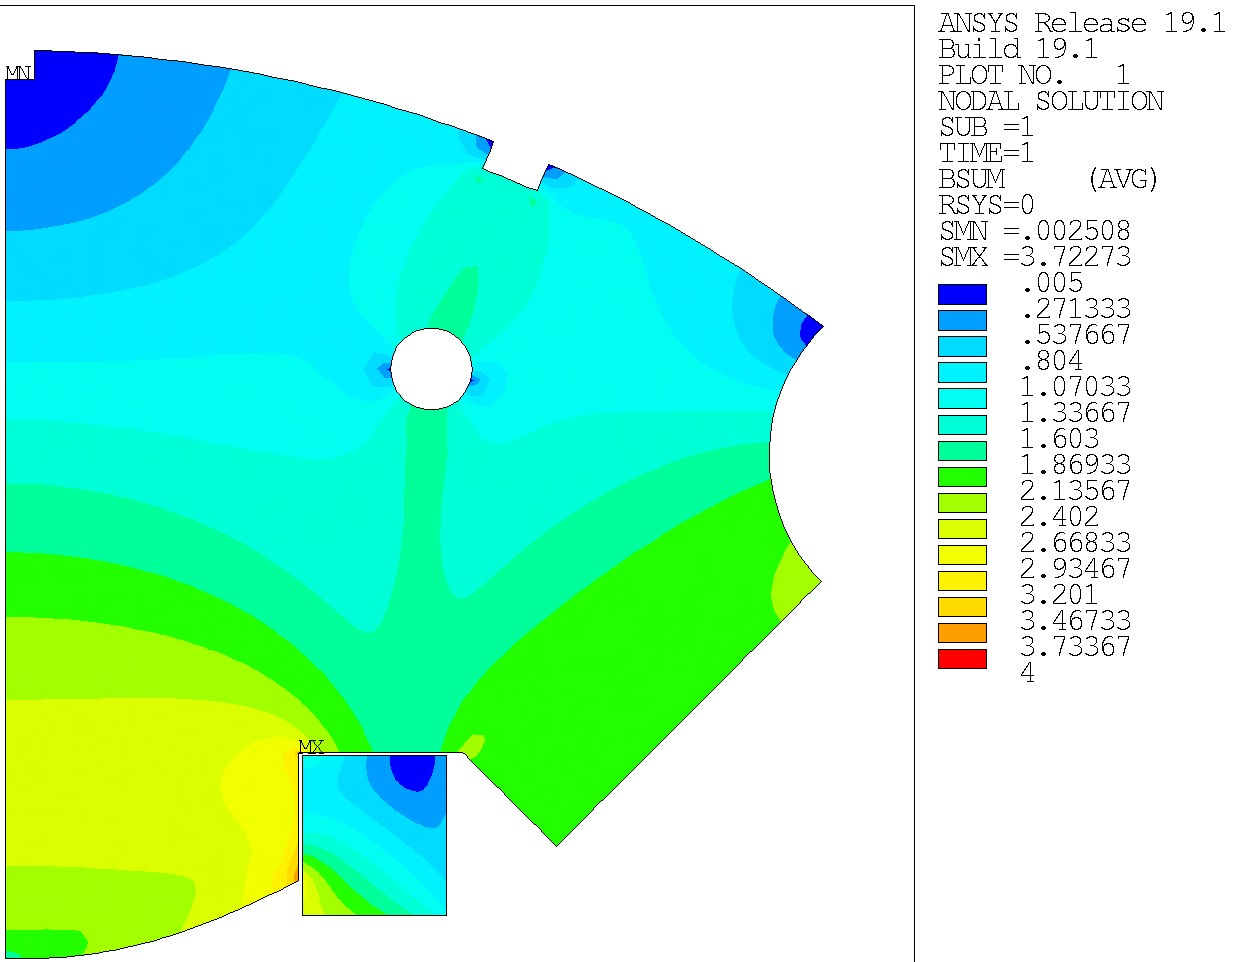
\includegraphics[width=.39\textwidth]{sections/skew_quad_q_det/figures/magnetic_map/peak_field_yoke_coil_current_86.jpg}};
    \end{tikzpicture}
    \caption{Magnetic field distribution in the coil and the iron yoke for $I=40~\text{A}$ (left) and $I=86~\text{A}$ (right).}
    \label{fig:skew_quad_magnetic_results_geometry_ansys}
\end{figure}

Figure~\ref{fig:skew_quad_magnetic_results_coil_ansys} presents the magnetic field distribution only in the coil for two values of transport current. In order to use the results from the coil for the quench velocity-based approach, the vector sum of the magnetic flux density is extracted at corner nodes of the coil elements. The magnetic field is linearly interpolated in the $(x,y)$-space for the current levels between the actually simulated values. 

\begin{figure}[H]
    \centering
    \begin{tikzpicture}
    \node at (0,0) {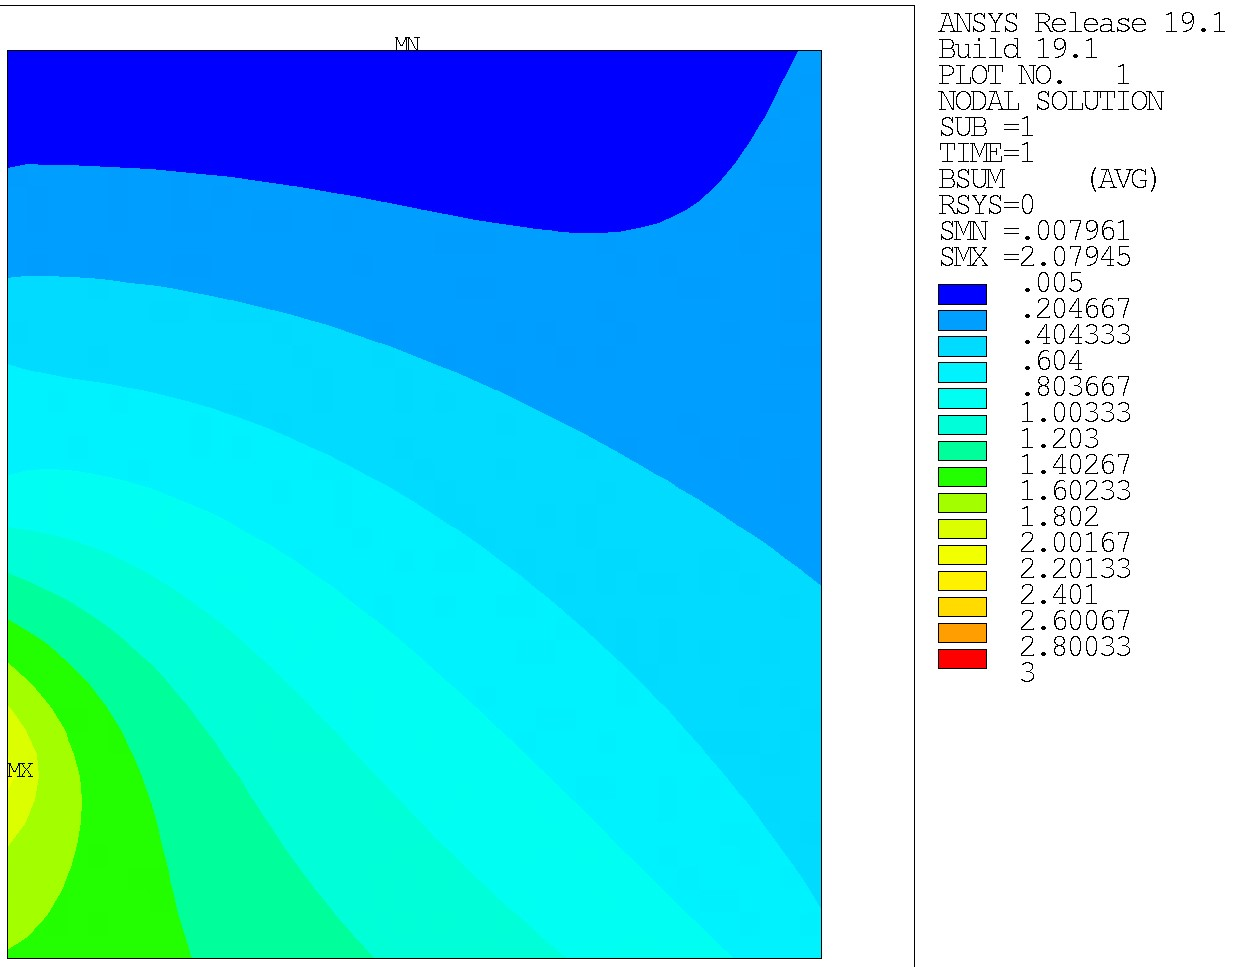
\includegraphics[width=.39\textwidth]{sections/skew_quad_q_det/figures/magnetic_map/peak_field_coil_current_40.jpg}};
    \node at (7.5,0) {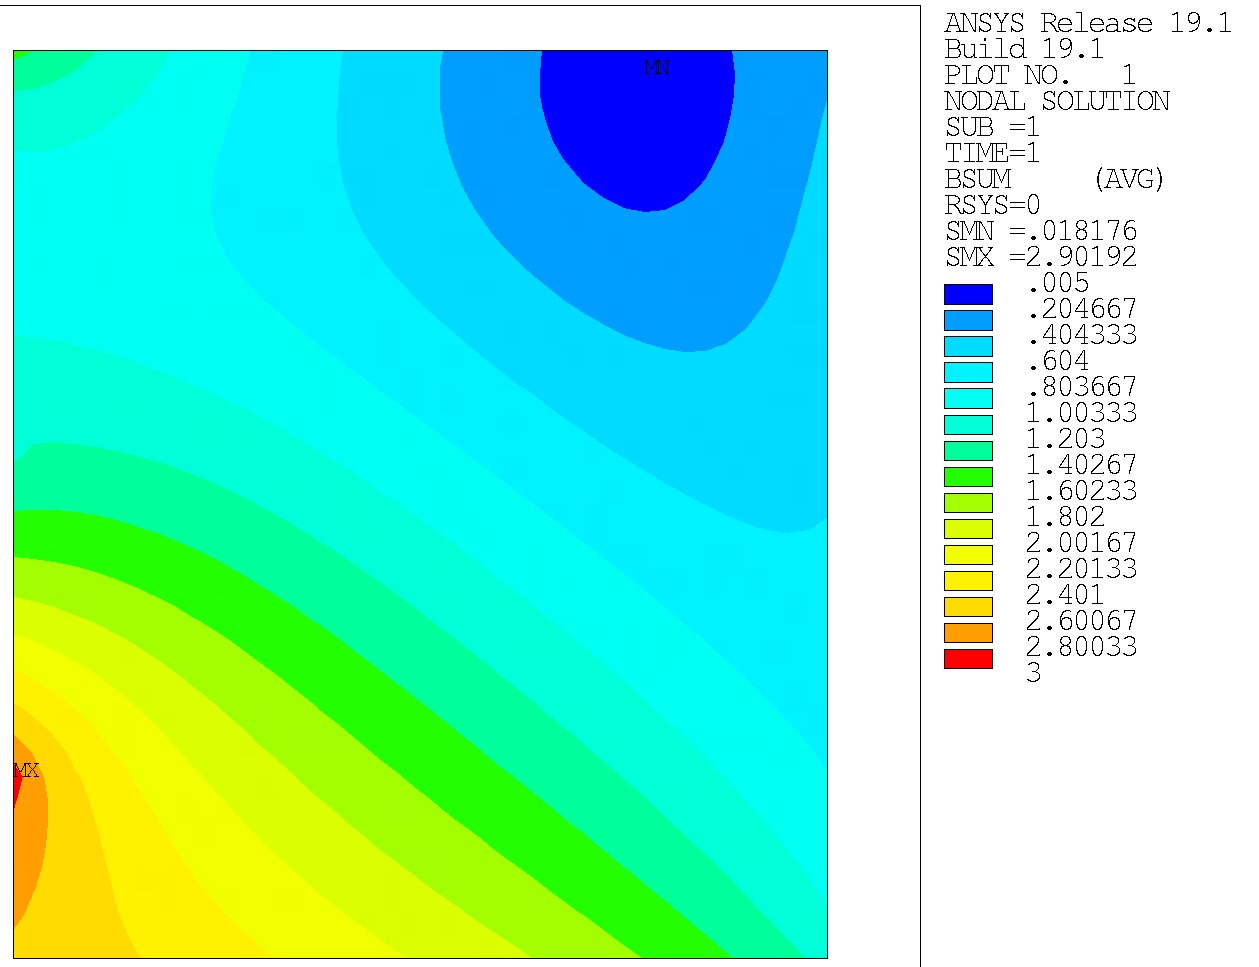
\includegraphics[width=.39\textwidth]{sections/skew_quad_q_det/figures/magnetic_map/peak_field_coil_current_86.jpg}};
    \end{tikzpicture}
    \caption{Magnetic field distribution in the coil for $I=40~\text{A}$ (left) and $I=86~\text{A}$ (right).}
    \label{fig:skew_quad_magnetic_results_coil_ansys}
\end{figure}

Figure~\ref{fig:skew_quad_magnetic_interpolation_coil_ansys} illustrates the magnetic field map applied to 754 windings for the nominal current of $I=86~\text{A}$. The central position of each winding is used to interpolate the magnetic field from the ANSYS results presented in Fig.~\ref{fig:skew_quad_magnetic_results_coil_ansys}. As current changes in time during the discharge process, the magnetic field of each winding varies with its position in the $(x,y)$-space.

\begin{figure}[H]
    \centering
    \begin{tikzpicture} [scale=0.8]
    
    \node[scale=0.8] at (0,0) {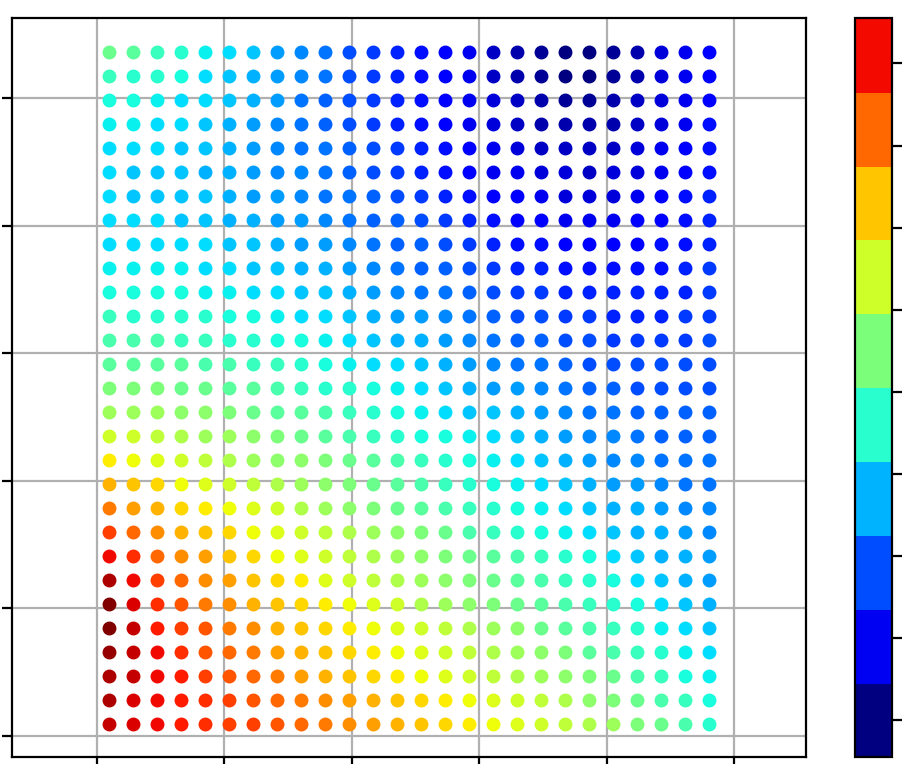
\includegraphics[width=.5\textwidth]{sections/skew_quad_q_det/figures/magnetic_map/Mag_field_distribution.png}};
    
    \node[black, scale=0.8] at (-3,-3.5) {0};
    \node[black, scale=0.8] at (-4.1,-2.95) {0};
    \node[black, scale=0.8] at (2.35,-3.6) {25};
    \node[black, scale=0.8] at (-4.1,2.45) {25};
    
    \node[black, scale=0.8] at (4.35,-2.82) {0.039};
    \node[black, scale=0.8] at (4.35,-2.2) {0.336};
    \node[black, scale=0.8] at (4.35,-1.5) {0.634};
    \node[black, scale=0.8] at (4.35,-0.8) {0.931};
    \node[black, scale=0.8] at (4.35,-0.1) {1.229};
    \node[black, scale=0.8] at (4.35,0.6) {1.526};
    \node[black, scale=0.8] at (4.35,1.3) {1.824};
    \node[black, scale=0.8] at (4.35,2) {1.121};
    \node[black, scale=0.8] at (4.35,2.7) {2.419};
    
    \node[black, scale=0.8] at (-0.225,-4) {$x$, mm (layers direction)};
    \node[black, rotate=90, scale=0.8] at (-4.75,0) {$y$, mm (layers direction)};
    \node[black, rotate=90, scale=0.8] at (5.3,0) {Magnetic field, T};

    \end{tikzpicture}
    \caption{Magnetic field distribution in the coil at $I=86~\text{A}$ applied separately to each winding.}
    \label{fig:skew_quad_magnetic_interpolation_coil_ansys}
\end{figure}

It is important to emphasise that ANSYS APDL allows for creating the material properties only as a function of a single-dependent variable (in this case temperature). It is not possible to include the dependence of material properties on the magnetic field in a relatively simple manner in this tool. The only possible method to add an additional variable in the repository of the material properties is to replace the repository at a certain moment of a transient simulation. The update of material properties is conducted at the communication time windows $t_\text{com}$ at which Python communicates with ANSYS to update the quench position in the coil. Since the update of the material properties is a time-consuming process, it is not recommended to perform it at each communication time window $t_\text{com}$ when hundreds of windings are modelled.